\section{Dataset and Task}

We conduct experiments on two datasets, the details for which are given below.

\subsection{Yelp Service Reviews}

The model is tested on a subset of the Yelp review dataset \citep{challenge2013yelp} and has been sourced from the code repository accompanying the implementation of the paper by \cite{shen2017style} open-sourced by the authors~\footnote{\url{https://github.com/shentianxiao/language-style-transfer}}. It contains 444101, 126670 and 63483 sentences for train, validation, and test, respectively, each sampling accompanied by binary sentiment labels. The maximum sentence length is 15, and the vocabulary size is about 9200.

\subsection{Amazon Product Reviews}

The model is trained and tested on an Amazon product reviews data-set~\footnote{\url{http://jmcauley.ucsd.edu/data/amazon/}}, following \cite{fu2017style}. The reviews were sourced from the code repository accompanying the paper~\footnote{\url{https://github.com/fuzhenxin/text_style_transfer}}. It contains 559142, 2000, 2000 sentences for train, validation, and test, respectively, each sampling accompanied by binary sentiment labels. The maximum sentence length is 20, and the vocabulary size is about 58000.


\section{Implementation Details and Model Hyper-parameters}

We implement the neural-network model in Tensorflow \citep{abadi2016tensorflow}, and utilize Scikit-learn \cite{pedregosa2011scikit} for latent-space classification evaluation metrics.

One of the most challenging aspects of training a variational autoencoder (VAE) is avoiding posterior collapse. In previous work \citep{yang2017improved, bowman2016generating, bahuleyan2017variational}, this has been done using manually crafted annealing schedules for weight of the KL-divergence term. We utilize the $\tanh$ annealing schedule proposed by \cite{bahuleyan2017variational}, and also use their technique of appending the latent vector ($[\bm s; \bm c]$) to the hidden state of the recurrent decoder at each time-step of decoding. Greedy decoding is utilized to predict the next word at each time-step.

The model uses style embeddings of size $8$ and content embeddings of size $128$ by default. The encoder and decoder are both GRU-RNNs with a size of $256$. The recurrent dropout probability for units in the encoder and decoder is $0.2$, and the same dropout probability is used for units in fully-connected layers as well.

We use the the Adam optimizer \citep{kingma2014adam} with an initial learning rate of $10^{-3}$ and train the model for 20 epochs. Both the autoencoder and its adversary are trained once per epoch with $\lambda_\text{mult} = 1$, and $\lambda_\text{adv} = 0.3$ and $\lambda_\text{badv} = 0.0001$.


\section{Evaluation Metrics} \label{sec:evaluation-metrics}

\subsection{Transfer Strength}

Transfer strength can be defined as a measure of how successful the model has been in generating sentences that are consistent with the attribute the needs to be transferred into them. This can be formulated as a Natural Language Understanding (NLU) task that takes in a sentence as input and predicts the presence of an attribute that we train the model to transfer.

Consistent with the approach taken in \cite{hu2017toward}, \cite{shen2017style} and \cite{fu2017style}, we train a separate model that learns to predict the class among the different classes to which transfer is possible. We use an open source implementation of the work presented by \cite{kim2014convolutional}, which is a convolutional neural network (CNN) model used for text classification, and build it into our model using an open-source implementation as a reference~\footnote{\url{https://github.com/dennybritz/cnn-text-classification-tf}}. This model has frequently been used as a text classification baseline to compare against \citep{tai2015improved} \citep{kiros2015skip} \citep{zhang2015character}.

This CNN classifier is trained on the entire corpus described in the previous section, with a held out validation set to assess improvements in accuracy over time. The test set for this classifier are the style-transferred sentences generated from the autoencoder model.

The style transfer strength is the ratio of sentences successfully transferred to the target style, to the total number of test sentences.
\begin{equation*}
	\text{transfer-strength} = \frac{count(\text{generated sentences with target style attribute})}{count(\text{generated sentences})}
\end{equation*}

Therefore, the optimal style transfer strength score is 1 and the worst is 0. Here, we choose to ignore the classification errors by our automated classification model, since a good model (with a high classification accuracy) would mis-classify approximately equal samples in each label, and a biased classifier would negatively impact the style transfer strength score.

The classifier we train achieves a classification accuracy of approximately 0.97 on the validation set used while training.

\subsection{Content Preservation} \label{ssec:content-preservation-metric}

The content preservation metric used by \cite{fu2017style} is also used in our work to judge content preservation of the generated sentences compared to the original. This metric is needed to ensure that the generated sentence doesn't talk about content, subjects or topics entirely different compared to the original sentence.

This method uses 100-dimensional GloVe embeddings \citep{pennington2014glove} pre-trained on the Wikipedia + GigaWord corpora~\footnote{\url{https://nlp.stanford.edu/projects/glove/}}. The min, mean and max GloVe word embeddings for each sentence are concatenated together to create a sentence representation. The cosine similarity between the source sentence and target sentence is used as a measure of content preservation.

Let $W$ be the set of word embeddings in a sentence $s$. Then the sentence embedding would be given by
\begin{equation*}
	\text{sentence-embedding} = [min(W);max(W);mean(W)]
\end{equation*}

Then the cosine similarity between two sentences $s_1$ and $s_2$ is obtained by
\begin{equation*}
	\text{cosine-similarity} = 1 - \cos(\text{sentence-embedding}_1, \text{sentence-embedding}_2)
\end{equation*}
where $\text{sentence-embedding}_1$ and $\text{sentence-embedding}_2$ are the sentence embeddings for $s_1$ and $s_2$ respectively. The mean cosine similarity of all the sentences in the test set is the content preservation that is reported for the experiment.

\begin{table}[ht]
	\centering
	\begin{tabular}{| p{0.45\linewidth} | p{0.45\linewidth} |}
		\hline
		\textbf{{Original (Positive)}}                                                      & \textbf{Transferred (Negative)}                  \\
		\hline
		\hline
		we had the shrimp with vegetables and shrimp fried rice both lovely                 & we had the bacon cheeseburger and it was cold    \\
		\hline
		both dishes prepared with quality veggies                                           & eggs benedict with no flavor                     \\
		\hline
		my appetizer was also very good and unique                                          & my steak was very dry and flavorless             \\
		\hline
		both times i have eaten the lunch buffet and it was outstanding                     & yes i have had the worst pizza i have ever had   \\
		\hline
		the new york eggrolls are outstanding and the beef dishes we ordered were flavorful & the main issue was our server was extremely rude \\
		\hline
	\end{tabular}
	\\
	\begin{tabular}{| p{0.45\linewidth} | p{0.45\linewidth} |}
		\hline
		\textbf{{Original (Negative)}}                                        & \textbf{Transferred (Positive)}        \\
		\hline
		\hline
		the chicken '' strip were paper thin oddly flavored strips            & the bread was wonderful as well        \\
		\hline
		the big chicken sandwich should be called the big mayonnaise sandwich & the salsa is the best i have ever had  \\
		\hline
		fries are not worth coming back                                       & prices are good                        \\
		\hline
		but honestly the worst hookah in las vegas                            & very authentic food in the east valley \\
		\hline
		second the service was terribly slow                                  & the sushi was delicious                \\
		\hline
	\end{tabular}
	\caption{Examples of poor content preservation while transferring sentiment}
	\label{tab:poor-content-preservation}
\end{table}

As seen in the examples above, it is easy to optimize for a style-transfer objective as long as there are no constraints on the content preservation regularization. To ensure this does not happen, we typically use a much larger content latent space than style latent space, as well as add the necessary regularizations discussed in the previous chapter.

Similar to \cite{fu2017style}, for the sentiment task, we exclude words from a sentiment lexicon \citep{hu2004mining} while evaluating the content preservation score.

However, a drawback of this content preservation metric devised by \cite{fu2017style} is that it can take a smaller range of possible values. The maximum content preservation value achievable is 1, but from empirical experiments performed by matching random pairs of sentences, the content preservation is $0.7591 \pm 0.0004$. This can be treated as an approximate lower bound on the metric for model assessment.

\subsection{Word Overlap}

In addition to the content preservation metric described above, we also utilize a simpler unigram overlap metric. Given a source sentence $x$ and a attribute style transferred sentence $y$, let $w_x$ and $w_y$ be the set of unique words present in $x$ and $y$ respectively. Then, the word overlap score can be calculated using
\begin{equation*}
	\text{word-overlap} = \frac{count(w_x \cap w_y)}{count(w_x \cup w_y)}
\end{equation*}
which is simply a normalized measure of overlapping unigrams in the source and target.

Theoretically, the word overlap score ranges from 0 to 1. However, in practice, since the expectation is that some words will be changed due to the style-transfer process, we wish to strike a good-balance with respect to the style transfer strength and original content preservation. Using experiments on random pairs of sentences, the word overlap score computed is $0.0098 \pm 0.0006$, which can again, be treated as a more realistic approximate lower-bound on this metric.

Word overlap can be used interchangeably with the 'Content Preservation' metric described above. For the experiments in this work, we report both.

\subsection{A note about Cycle Consistency Loss}

The cycle consistency loss is described in the image domain-adaptation work done by \cite{zhu2017unpaired}. Given domains $X$ and $Y$, They aim to learn a mapping similar to ours, $G: X \rightarrow Y$ which transfers attributes of $X$ to $Y$. At the same time, they also learn an inverse mapping $F: Y \rightarrow X$. The cycle consistency loss is the step that pushes $F(G(X)) \approx X$ and $G(F(Y)) \approx Y$, as shown in Figure \ref{fig:cycle-consistency}.

\begin{figure}[ht]
	\centering
	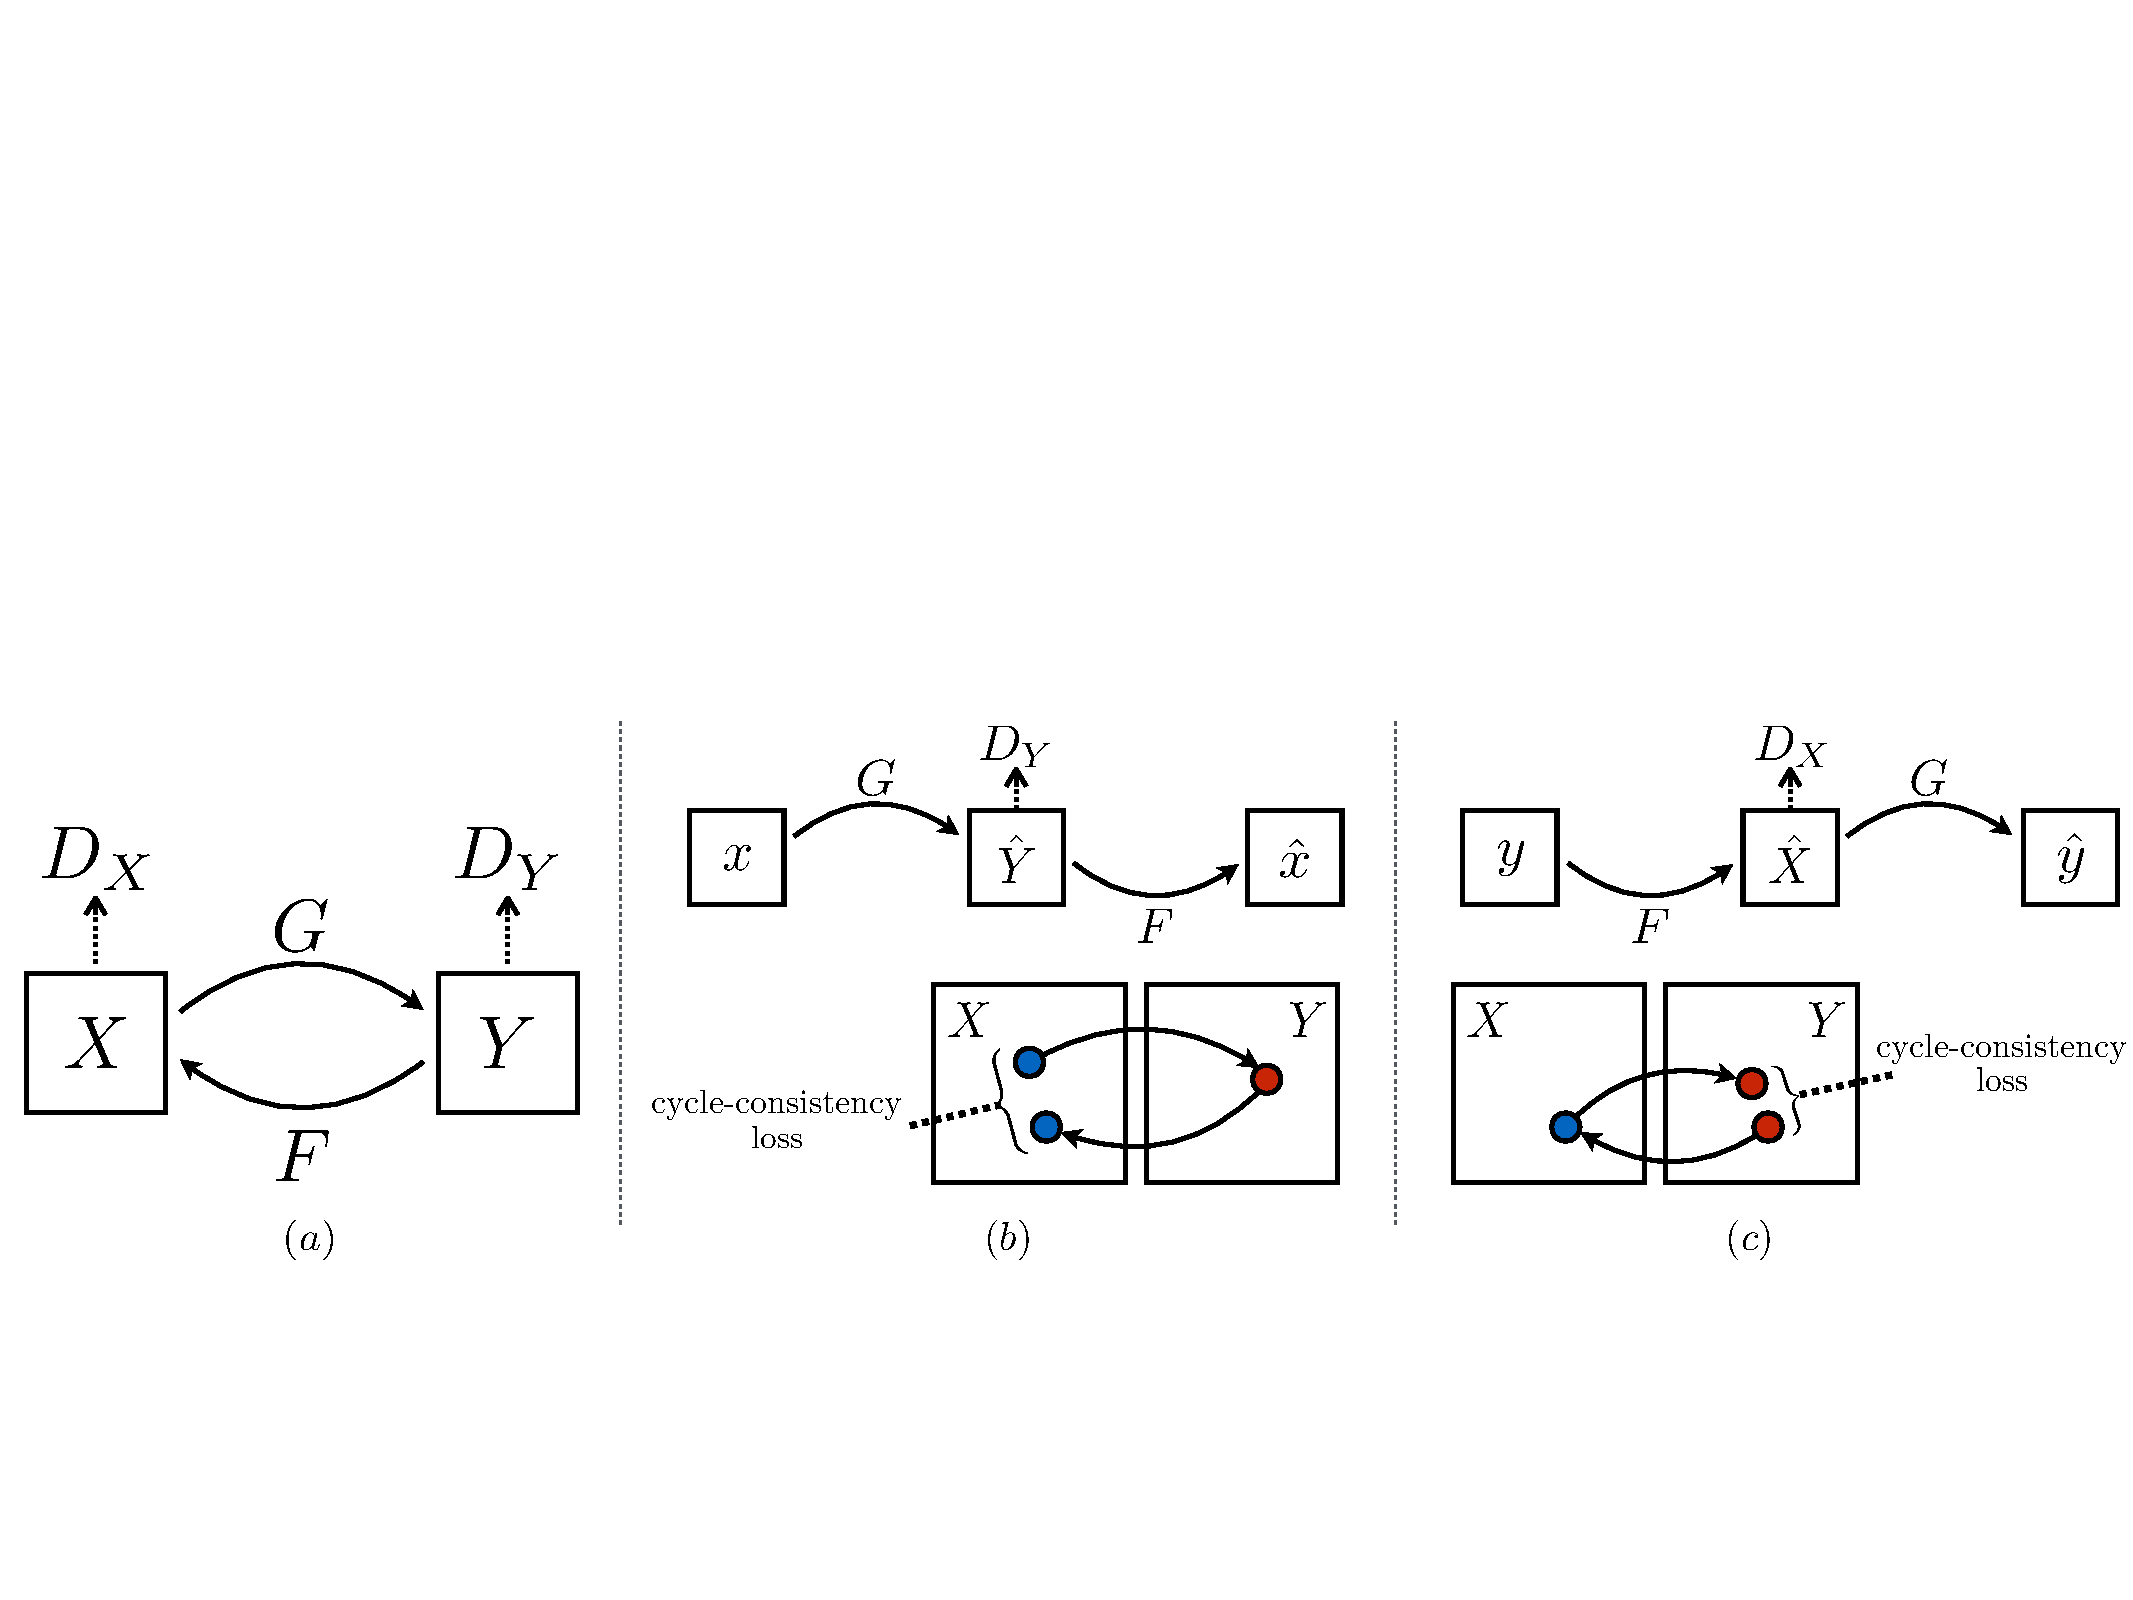
\includegraphics[width=\textwidth]{images/cycle-consistency}
	\imgsrc{\cite{zhu2017unpaired}}
	\caption{\label{fig:cycle-consistency} Cycle Consistency Loss}
\end{figure}

This training routine could also be used as an evaluation metric for other domain adaptation tasks, like text attribute style transfer. The advantage of using a cycle consistency loss is that no other content preservation metric is needed, and no domain or style specific lexicons would be needed.

In the case of our model, assume that, for a sample sentence $x$ from the domain $X$ and the ideal equivalent sentence transferred to the domain $Y$ is $y$. The transferred sentence generated by our model is $\hat{y}$. In the above approaches we compare $\hat{y}$ with the original $x$ using a content similarity metric. However, if the cycle consistency loss were to be used, we can further transfer the style of the sentence $\hat{y}$ back to the domain $X$, obtaining $\hat{x}$. Now that we have two sentences in the same domain $x$ and $\hat{x}$, it is a lot simpler to compare them, and this can be achieved by traditional parallel corpora evaluation metrics like BLEU \citep{papineni2002bleu}.

However, in our problem, assuming a scenario in which both functions $F$ and $G$ do not successfully disentangle style and content, and transfer a content as well as style at inference time, like the examples presented in \ref{tab:poor-content-preservation}. In this case, the transformation could look like
\begin{equation*}
	x \xrightarrow{G} y^* \xrightarrow{F} x
\end{equation*}
where $y^*$ is a sentence with the requisite transferred style, as well as undesirable transferred content. Such examples would score highly on both the style transfer strength metric and the cycle consistency metric.

Hence, metric would not be able to tell the difference between a model with poor content preservation and a good model, and we refrain from using it in our evaluation.


\section{Experiment Results}

\subsection{Disentangling Latent Space}

We first analyse how the style (sentiment) and content of the latent space are disentangled. We train a softmax classifier from each latent space, style and content, alongside our autoencoder model and train it to predict the true class of an input sample. The results are shown in Table \ref{tab:latent-space-classification}. vae-The results reported here are for the Yelp dataset.

In our experiments, we use an 8-neuron layer for the style embedding and a 128-neuron layer for the content embedding. We see that the 128-dimensional content vector is not discriminative for style. It achieves a classification accuracy that is slightly better than random/majority guess. However, the 8-dimensional style vector $\bm s$, despite its low dimensionality, achieves significantly higher style classification accuracy. When combining content and style vectors, we achieve no further improvement. These results verify the effectiveness of our disentangling approach, because the content space doesn't contain style information, opposed to the style space.

\begin{table}[ht]
	\centering
	\begin{tabular}{| l | r | r |}
		\hline
		                                        & \textbf{Deterministic} & \textbf{Variational} \\
		\hline \hline
		Random/Majority guess                   & 0.6018                 & 0.6018               \\ \hline \hline
		Content latent space  ($\bm c$)         & 0.6137                 & 0.6567               \\ \hline
		Style latent space ($\bm s$)            & 0.7927                 & 0.7911               \\ \hline
		Complete latent space ($[\bm s;\bm c]$) & 0.7918                 & 0.7918               \\
		\hline
	\end{tabular}
	\caption{Style classification accuracy}
	\label{tab:latent-space-classification}
\end{table}


The latent space can also be visualized with our method since we are able to infer a pair of style and content embeddings for every training data sample. We use t-SNE plots \cite{maaten2008visualizing} and use a random sample from each label to plot both the style and content embeddings inferred for them during a given epoch of the training procedure. Our hypothesis is that while the points for different labels plotted in the content embedding space would be mixed and indistinguishable in terms of plot co-ordinates, the style embedding space would display the opposite characteristic and show a clean separation of samples from each label.

We T-SNE show plots of both and deterministic autoencoder (DAE) and variational autoencoder (VAE) models in Figure \ref{fig:dae-tsne} and Figure \ref{fig:vae-tsne}, respectively.

\begin{figure}[ht]
	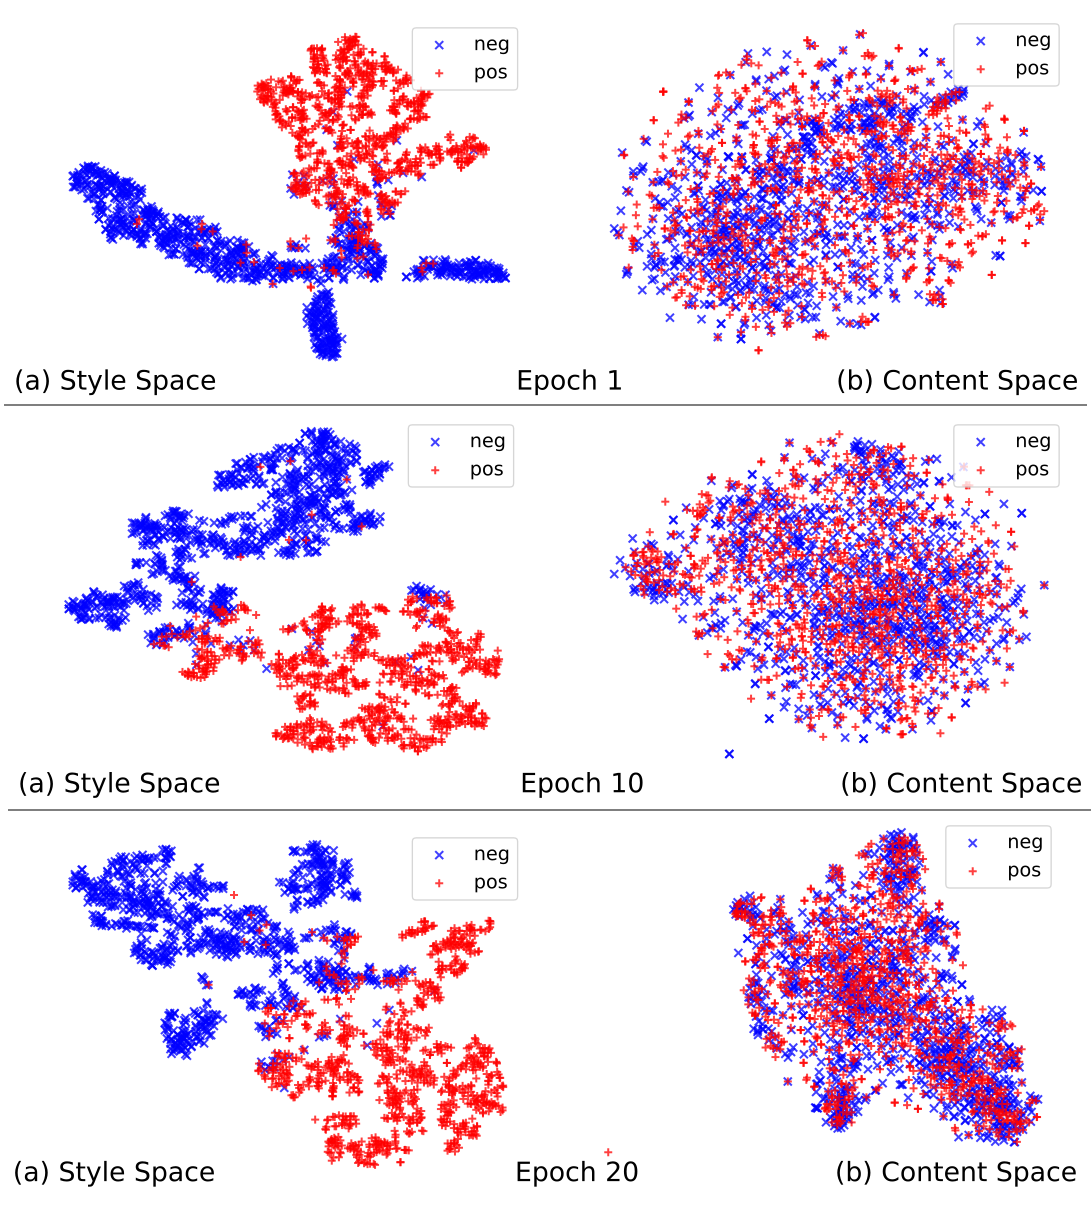
\includegraphics[width=\linewidth]{images/dae-latent-spaces}
	\caption{t-SNE plots of (a) style and (b) content spaces in the DAE model}
	\label{fig:dae-tsne}
\end{figure}

\begin{figure}[ht]
	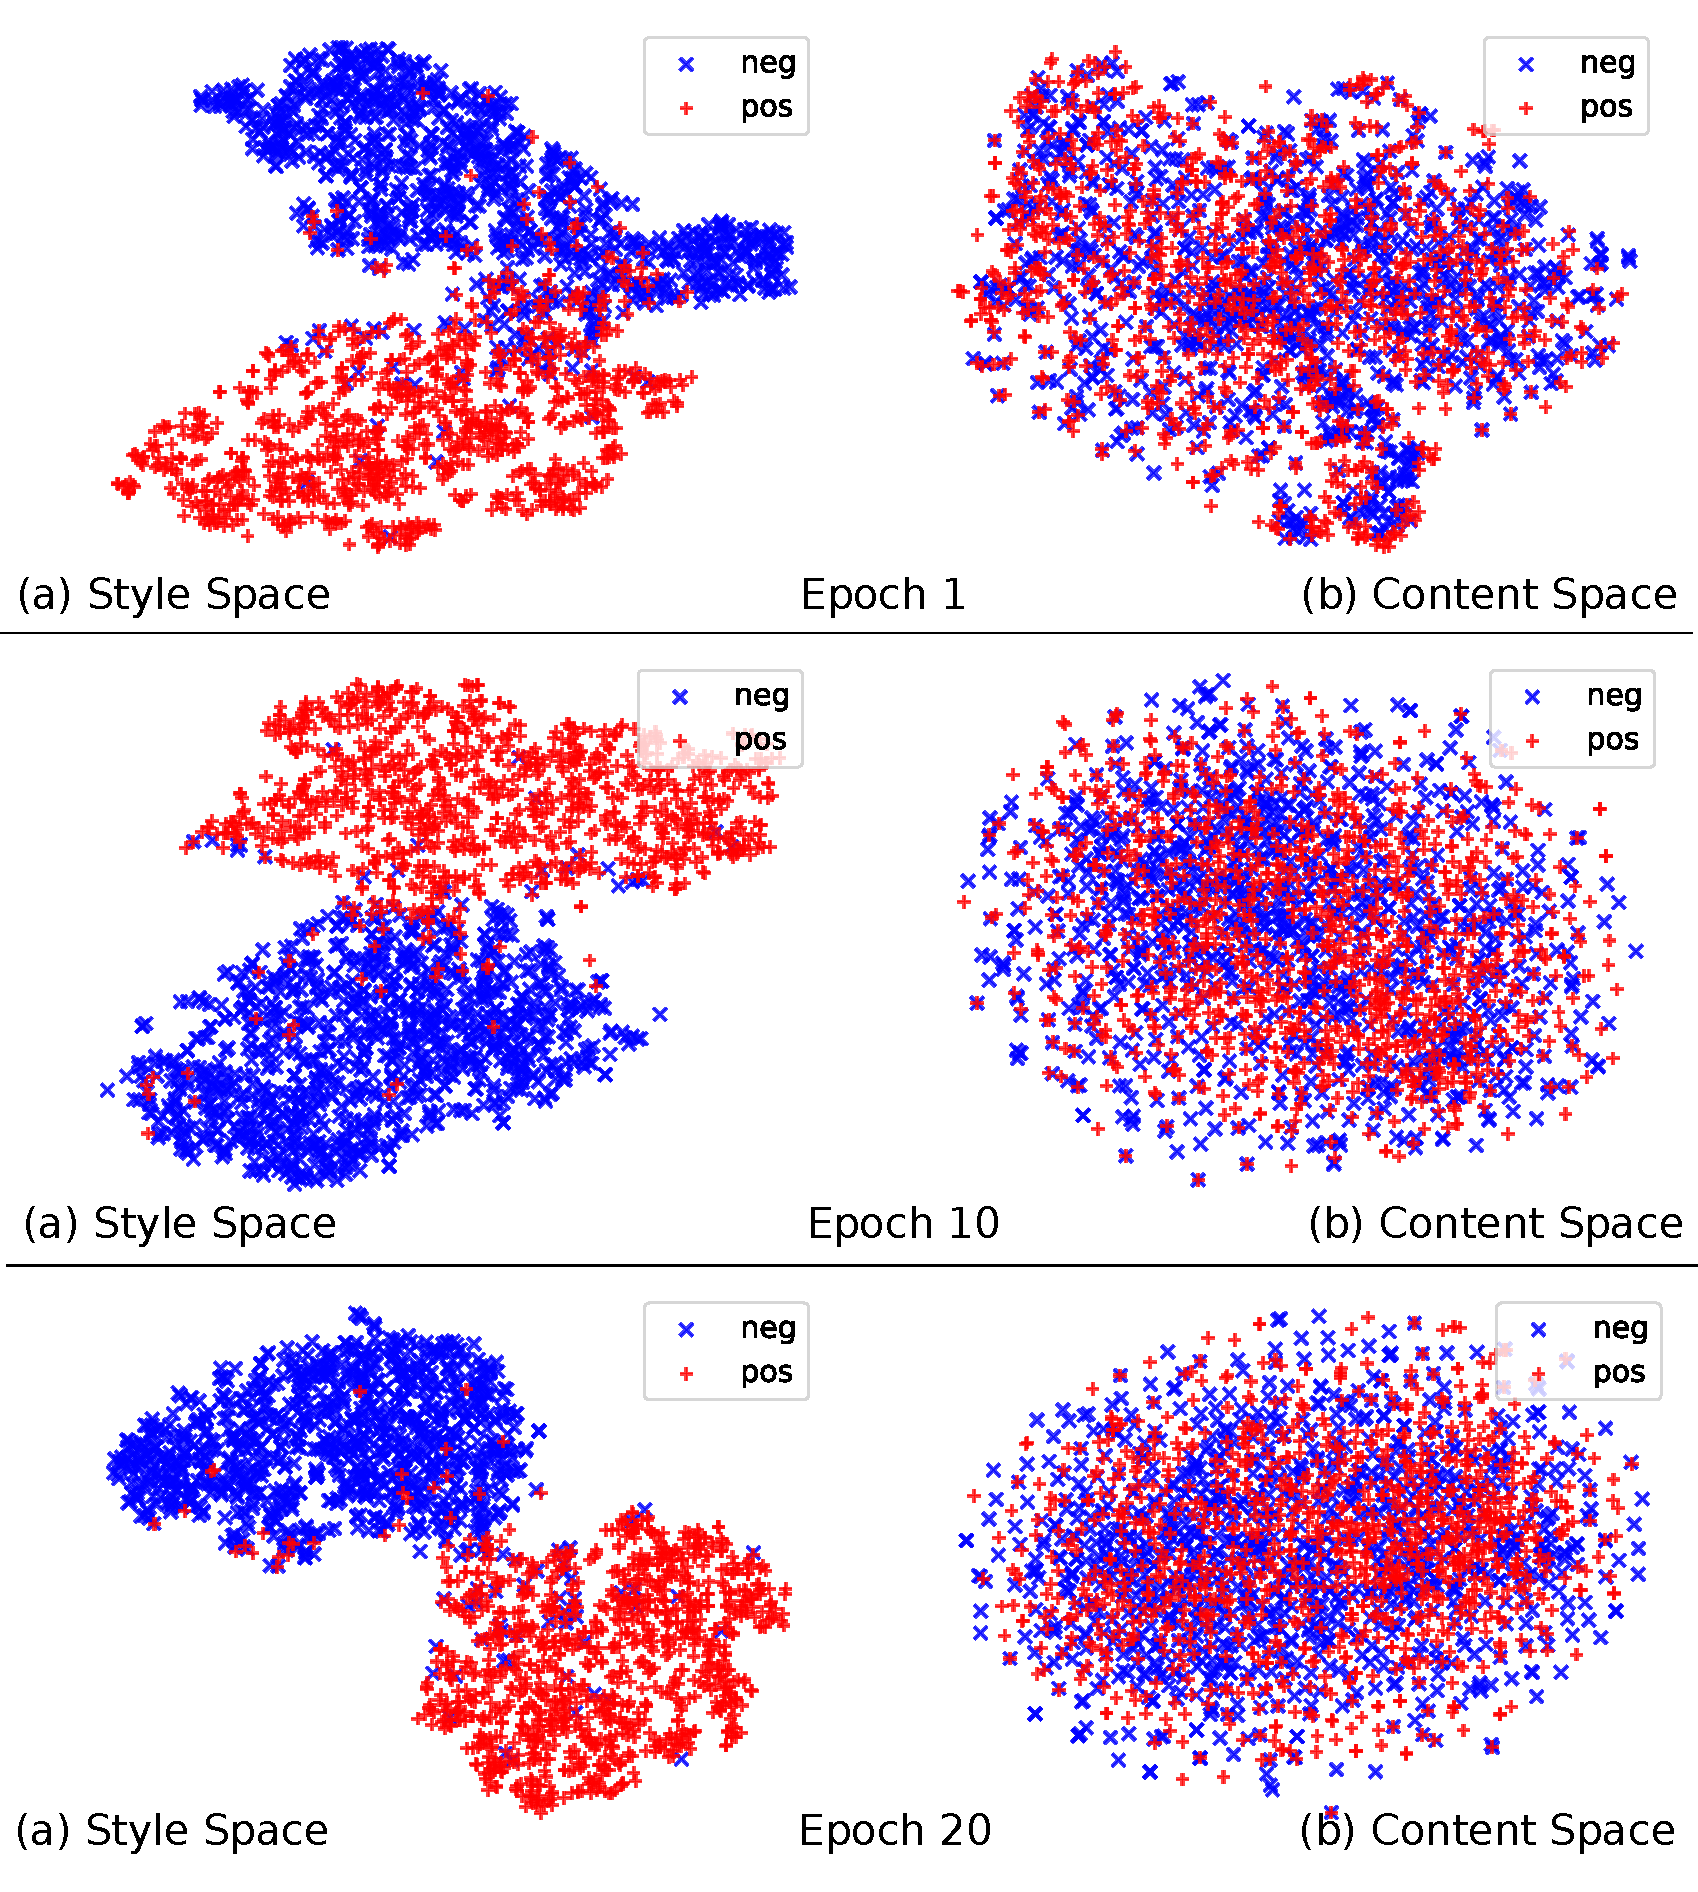
\includegraphics[width=\linewidth]{images/vae-latent-spaces}
	\caption{t-SNE plots of (a) style and (b) content spaces in the VAE model}
	\label{fig:vae-tsne}
\end{figure}

As can be seen from the plots, sentences with different styles are noticeably separated in a cleaner manner in the style space (LHS), but are indistinguishable in the content space (RHS). It is also evident that the latent space learned by the variational autoencoder is significantly smoother and continuous than the one learned by the deterministic autoencoder. Since we are essentially given the decoder a previously unseen combination of style and latent space at inference time, our hypothesis is that using a variational autoencoder would lead to more fluent generated sentences.


\subsection{Style-Transferred Text Generation}

We apply the disentangled latent space to a style-transfer sentence generation task, where the goal is to generate a sentence with different sentiment (style). We use the metrics discussed in \ref{sec:evaluation-metrics} to evaluate our models.

We compare our approach with state-of-the-art previous work in Table \ref{tab:comparison-previous}. We re-conducted the experiments with their publicly available code and data.

Results show that, our approach achieves a comparable content-preservation score to previous work, but a significantly better style-transfer score, showing that our disentangled latent space can be used for better style-transfer sentence generation.

\begin{table}[ht]
	\centering
	\begin{tabular}{| l | r | r | r |}
		\hline
		\multirow{2}{*}{
		\textbf{Model}}                       & \textbf{Style}    & \textbf{Content}      & \textbf{Word}    \\
		                                      & \textbf{Transfer} & \textbf{Preservation} & \textbf{Overlap} \\
		\hline
		\hline
		Cross-alignment \citep{shen2017style} & 0.8086            & 0.8919                & 0.2086           \\
		\hline
		Style Embedding \citep{fu2017style}   & 0.1819            & 0.9585                & 0.6661           \\
		\hline
		Ours (DAE)                            & 0.8425            & 0.8924                & 0.2551           \\
		Ours (VAE)                            & 0.8903            & 0.8824                & 0.2105           \\
		\hline
	\end{tabular}
	\caption{Comparison with previous approaches on the Yelp Dataset}
	\label{tab:comparison-previous}
\end{table}


Table \ref{tab:ablation-results} presents the results of an ablation test. We see that both, the adversarial loss and multi-task losses, play a role in the strength of style transfer. It also shows that their usage in a combination can further boost performance of the style-transfer strength.

\todo[inline]{Update ablation tests table with latest results}

\begin{table}[ht]
	\centering
	\begin{tabular}{| l | r | r |}
		\hline
		\textbf{Training Objectives}                                                  & \textbf{Style Transfer} & \textbf{Content Preservation} \\
		\hline
		\hline
		$\mathcal{L}_\text{rec}$                                                      & 0.5053                  & 0.9103                        \\
		\hline
		$\mathcal{L}_\text{rec}$, $\mathcal{L}_\text{adv}$                            & 0.5901                  & 0.9121                        \\
		\hline
		$\mathcal{L}_\text{rec}$, $\mathcal{L}_\text{mult}$                           & 0.6445                  & 0.9053                        \\
		\hline
		$\mathcal{L}_\text{rec}$, $\mathcal{L}_\text{adv}$, $\mathcal{L}_\text{mult}$ & 0.7708                  & 0.8958                        \\
		\hline
	\end{tabular}
	\caption{Ablation tests}
	\label{tab:ablation-results}
\end{table}

Some examples of style-transfer sentence generation are illustrated in Table \ref{tab:transfer-samples}. We see that, with the empirically estimated style vector, we can flexibly control the sentiment of generated sentences.

\todo[inline]{Update text samples table with latest results}

\begin{table}[ht]
	\centering
	\begin{tabular}{| p{0.45\linewidth} | p{0.45\linewidth} |}
		\hline
		\textbf{{Original}}                                                        & \textbf{Transferred (Positive $\rightarrow$ Negative)}                    \\
		\hline
		\hline
		i bought this cuisipro mister to replace my old mister last june-(number)  & i bought this a couple of times and was disappointed in this product      \\
		\hline
		quality is good, recevied in time and works as expected.                   & quality is good but i am returning it                                     \\
		\hline
		all in all, i am very happy with this headset.                             & all in all i was expecting a good product                                 \\
		\hline
		\hline
		\textbf{{Original}}                                                        & \textbf{Transferred (Negative $\rightarrow$ Positive)}                    \\
		\hline
		\hline
		i sent it back and requested a refund, and never got the refund.           & i sent it back and gave it a try and it works great                       \\
		\hline
		so i tried just one (number) piece each n still the same results.          & so i bought the two sizes and the other ones are great                    \\
		\hline
		i am going to buy a replacement and wish i had sent this back for a refund & i am going to go through the same time and i have been using it for years \\
		\hline
	\end{tabular}
	\caption{Examples of style-transferred text generation}
	\label{tab:transfer-samples}
\end{table}
